\documentclass[aspectratio=169]{beamer}

%\includeonlyframes{current}

\usepackage[utf8]{inputenc}
\usepackage[american]{babel}
\usepackage{amsmath,amsthm}
\usepackage{unicode}
\usepackage{booktabs}
\usepackage{ifthen}
\usepackage{tikz}
\usetikzlibrary{calc,arrows,arrows.meta,intersections,positioning,decorations.markings}
\usepackage{ulem}

\mode<presentation>{%
  \usetheme{ibm}
}

\newcommand{\Z}{ℤ}
\newcommand{\F}{\mathbb{F}}
\renewcommand{\a}{\mathfrak{a}}
\renewcommand{\b}{\mathfrak{b}}
\newcommand{\g}{\mathfrak{g}}
\newcommand{\G}{\mathcal{G}}
\newcommand{\E}{\mathcal{E}}
\newcommand{\End}{\operatorname{End}}
\newcommand{\Hom}{\operatorname{Hom}}
\newcommand{\M}{\mathcal{M}}
\newcommand{\fp}{\mathrm{fp}}
\DeclareMathOperator{\rank}{rank}
\newcommand{\Cl}{\operatorname{Cl}}
\newcommand{\GL}{\operatorname{GL}}
\newcommand{\SL}{\operatorname{SL}}
\renewcommand{\O}{\mathcal{O}}

\title{Isogeny-based Cryptography}
\author{Luca De Feo}
\date{December 14, 2025, Indocrypt}
\institute{IBM Research Zürich}

\begin{document}

\frame[plain]{\titlepage}

%%

\begin{frame}{Are you quantum-safe?}
  \centering
  \includegraphics[height=0.7\textheight]{qc-color}
\end{frame}

%%

\begin{frame}
  \Large
  \begin{tikzpicture}[remember picture,overlay,shift={(current page.center)},xscale=0.5]
    \fill[white] (0,8) -- (16,8) -- (16,-8) -- (0,-8);
    \fill[ibmblue] (0,8) -- (-16,8) -- (-16,-8) -- (0,-8);
    
    \node[white,anchor=east] at (0,3.5) {\LARGE\bf Only two ways to};
    \node[ibmblue,anchor=west] at (0,3.5) {\LARGE\bf Post-quantum Encryption};
    
    \node[white,align=center] at (-8,0) {Noisy linear algebra:\\\normalsize Lattices, Codes};
    \node[ibmblue,align=center] at (8,0) {Far-fetched generalizations\\of the discrete logarithm:\\\normalsize Isogenies};
  \end{tikzpicture}
\end{frame}

%%

\begin{frame}{What crypto from isogenies?}
  \small
  \renewcommand{\arraystretch}{1.5}
  \begin{tabular}{p{0.15\textwidth} p{0.25\textwidth} p{0.25\textwidth} p{0.25\textwidth}}
    & \emph{Key exchange / Encryption} & \emph{Identification / Signature} & \emph{Other}\\
    \hline
    \emph{Quadratic}\par \emph{(Group actions)}
    & Couveignes--Rostovtsev--Stolbunov\par CSIDH\par SCALLOP
                                & SeaSign\par CSI-FiSh\par PEGASIS
                                                             & Threshold\par PAKE\par \dots\\
    \emph{Quaternionic}
    & ---
                                & \strut\emph{SQIsign}\par SIDH-like signatures
                                                             & Ring signatures\par Adaptor signatures\par Chameleon hash\par \dots\\
    \emph{\textit{Ad hoc}}
    & \strut\alert{SIDH~$\dagger$}\par SIDH fixes\par FESTA
                                & SIDH-like signatures
                                                             & Time-release crypto\par\dots
  \end{tabular}
\end{frame}


%%

\begin{frame}[plain]
  \begin{beamercolorbox}[sep=0.1px,center,wd=\paperwidth,sep=0.5\paperheight]{palette tertiary}
    \Huge\centering Cryptographic Group Actions
  \end{beamercolorbox}
\end{frame}

%%

\begin{frame}{A cyclic group}
  \Large
  \centering
  \begin{tikzpicture}
    \node at (0,0) {$G = \langle g\rangle$};
    
    \node (g) at (0:4) {$g$};
    \node (g2) at (30:4) {$g^2$};
    \node at (60:4) {$g^3$};
    \node at (-30:4) {$g^n = g^0 = 1$};
    
    \draw (5:4) arc (5:25:4) (35:4) arc (35:55:4) (-25:4) arc (-25:-5:4);
    \draw[dashed] (65:4) arc (65:325:4);
  \end{tikzpicture}
\end{frame}

%%

\begin{frame}{Diffie--Hellman key exchange}
  \begin{description}
  \item[Goal:] Alice and Bob have never met before. They are chatting
    over a public channel, and want to agree on a \emph{shared secret}
    to start a private conversation.
  \item[Setup:] They agree on a (large) cyclic group
    $G=\langle g\rangle$ of order $N$.
  \end{description}

  \begin{center}
    \begin{tikzpicture}
      \node at (0,0) {\bf Alice};
      \node at (7,0) {\bf Bob};
      \node at (0,-1) {pick random \alert{$a\inℤ/Nℤ$}};
      \node at (0,-1.5) {compute $A=g^a$};
      \node at (7,-1) {pick random \alert{$b\inℤ/Nℤ$}};
      \node at (7,-1.5) {compute $B=g^b$};
      \draw[->]
      (1,-2) to node[auto] {$A$} (6,-2);
      \draw[->] (6,-2.5) to node[auto] {$B$} (1,-2.5);
      \node at (3.5,-3.5) {\emph{Shared secret} is \alert{$B^a=g^{ab}=A^b$}};
    \end{tikzpicture}
  \end{center}
\end{frame}

%%

\begin{frame}{What's needed for key exchange?}
  \begin{columns}
    \begin{column}{0.5\textwidth}
      \centering
      \begin{tikzpicture}
        \begin{uncoverenv}<-3>
          \begin{scope}
            \def\crater{13}
            \def\jumpa{-8}
            \def\diam{2.5cm}

            \uncover<1>{
              \foreach \i in {1,...,\crater} {
                \draw[blue!20!white] (360/\crater*\i : \diam) to[bend right] (360/\crater*\i+360/\crater : \diam);
              }
            }

            \uncover<2->{
              \pgfmathparse{int(\crater/2)}
              \let\last\pgfmathresult
              \foreach \i in {1,...,\last} {
                \pgfmathparse{mod(pow(2,\i-1),\crater)}
                \let\e\pgfmathresult
                \draw[red] (360/\crater*\e : \diam) to[bend left] (360/\crater*\e*2 : \diam);
                \draw[red] (-360/\crater*\e : \diam) to[bend right] (-360/\crater*\e*2 : \diam);
              }
            }

            \uncover<3->{
              \pgfmathparse{int(\crater/2)}
              \let\last\pgfmathresult
              \foreach \i in {1,...,\last} {
                \pgfmathparse{mod(pow(6,\i-1),\crater)}
                \let\e\pgfmathresult
                \draw[blue] (360/\crater*\e : \diam) to[bend right] (360/\crater*\e*6 : \diam);
                \draw[blue] (-360/\crater*\e : \diam) to[bend left] (-360/\crater*\e*6 : \diam);
              }
            }
            
            \pgfmathparse{\crater-1}
            \let\last\pgfmathresult
            \foreach \i in {0,...,\last} {
              \draw[fill] (360/\crater*\i: \diam) circle (2pt) +(360/\crater*\i: 0.5) node{$g^{\i}$};
            }
          \end{scope}
        \end{uncoverenv}
        
        \begin{uncoverenv}<4->
          \begin{scope}
            \def\crater{12}
            \def\jumpa{5}
            \def\diam{2.5cm}

            \foreach \i in {1,...,\crater} {
              \draw[red,-latex] (360/\crater*\i : \diam) to[bend right] (360/\crater*\i+360/\crater : \diam);
              \draw[blue,-latex] (360/\crater*\i : \diam) to[bend right=10] (360/\crater*\i+\jumpa*360/\crater : \diam);
            }

            \foreach \i in {1,...,\crater} {
              \pgfmathparse{int(mod(pow(2,\i-1),\crater+1))}
              \let\e\pgfmathresult
              \draw[fill] (360/\crater*\i: \diam) circle (2pt) +(360/\crater*\i: 0.5) node{$g^{\e}$};
            }
          \end{scope}
        \end{uncoverenv}
      \end{tikzpicture}
    \end{column}
    \begin{column}{0.4\textwidth}
      The axioms of a dlog group:
      \begin{itemize}
      \item[\sout{prod:}] \sout{$g^ag^b = g^{a+b}$,}
      \item[exp:] $(g^a)^n = g^{na}$.
      \end{itemize}

      \bigskip
      The hard problem:
      \begin{itemize}
      \item[dlog:] $g^a \mapsto a$.
      \end{itemize}

      \bigskip
      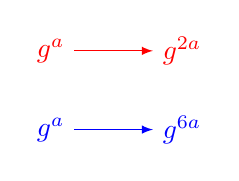
\begin{tikzpicture}
        \uncover<2->{\draw[red,-latex] (0,0) node[anchor=east]{$g^a$} -- (1,0) node[anchor=west] {$g^{2a}$};}
        \uncover<3->{\draw[blue,-latex] (0,-1) node[anchor=east]{$g^a$} -- (1,-1) node[anchor=west] {$g^{6a}$};}
      \end{tikzpicture}
    \end{column}
  \end{columns}
\end{frame}

%%

\begin{frame}{Symmetries = Group action}
  \centering
  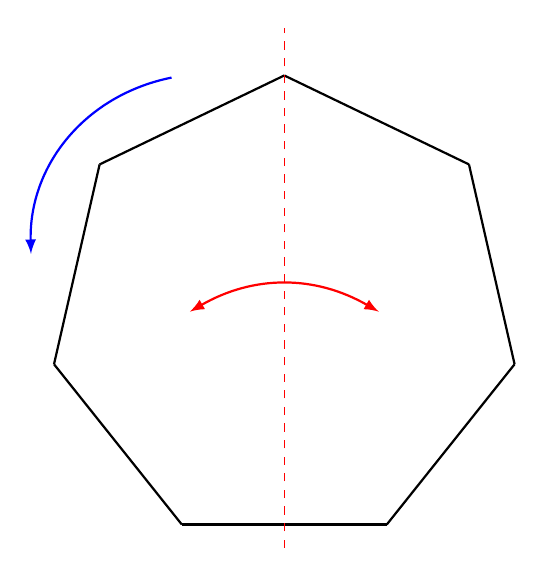
\begin{tikzpicture}[scale=3,rotate=90]
    \def\n{7}
    \foreach \i in {1,...,\n} {
      \draw[thick] (\i*360/\n:1) -- ({(\i+1)*360/\n}:1);
    }
    \draw[red,dashed] (-1,0) -- (1.2,0);
    \draw[red,latex-latex,thick] (0,-0.4) to[bend right] (0,0.4);
    \draw[blue,-latex,thick] (0.5*360/\n:1.1) to [bend right=40] (1.5*360/\n:1.1);
  \end{tikzpicture}
\end{frame}

%%

\begin{frame}
  \begin{block}{Group action}
    \emph{$\G\circlearrowright\E$}: A (finite) set $\E$ \emph{acted
      upon} by a group $\G$ \emph{freely} and \emph{transitively}:
    \begin{align*}
      * : \G × \E &→ \E\\
      \g * E &↦ E'
    \end{align*}
    \par\begin{description}
    \item[Compatibility:] \emph{$\g' * (\g * E) = (\g'\g)*E$} for all
      $\g,\g'\in\G$ and $E\in\E$;
    \item[Identity:] \emph{$\mathfrak{e} * E = E$} if and only if
      $\mathfrak{e}\in\G$ is the identity element;
    \item[Regularity:] for all $E,E'\in\E$ there exist a \emph{unique
        $\g\in\G$} such that \emph{$\g*E'=E$}.
      \setlength{\itemsep}{2em}
    \end{description}
  \end{block}
\end{frame}

%%

\begin{frame}{Cryptographic Group Actions \small(Alamati, D., Montgomery, Patranabis 2021)}
  \begin{block}{Hard Homogeneous Space (HHS) --- Couveignes 1997 \small(eprint:2006/291)}
    \emph{$\G\circlearrowright\E$} such that $\G$ is commutative and:
    \begin{itemize}
    \item \emph{Evaluating} $E' = \g*E$ is \emph{easy};
    \item \emph{Inverting} the action is \emph{hard}.
    \end{itemize}
  \end{block}

  \begin{block}{Example}
    Let $G$ be a group of order $13$, then \emph{$(\Z/13\Z)^\times \circlearrowright G$} defined by
    \[a * g := g^a\]
    is an HHS\dots\pause
    But
    \[\alert{g^a \cdot g^b = g^{a+b}}\]
    has no interpretation as a group action!
  \end{block}
\end{frame}

%%

\begin{frame}{Key exchange from group actions}
  \begin{description}
  \item[Public parameters:] A \emph{HHS $\G\circlearrowright \E$} of
    order $N$ (large, but not necessarily prime).
  \end{description}

  \bigskip
  
  \begin{center}
    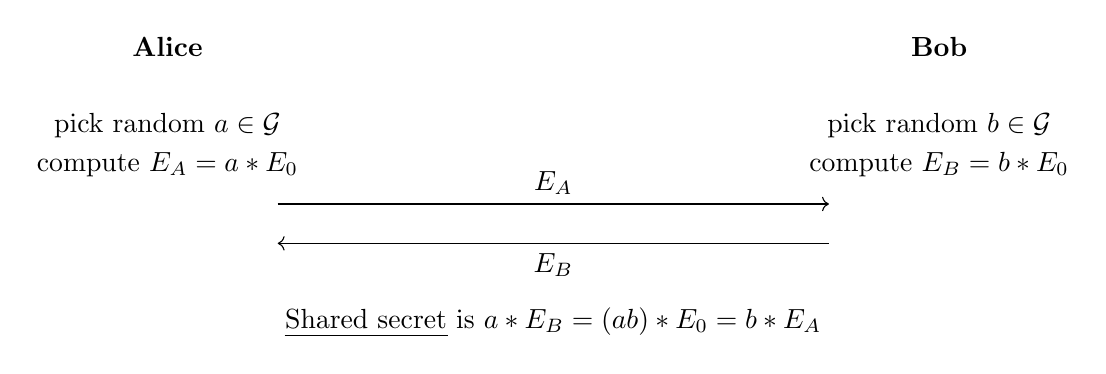
\begin{tikzpicture}[x=1.4cm]
      \node at (0,0) {\bf Alice};
      \node at (7,0) {\bf Bob};
      \node at (0,-1) {pick random \alert{$\a\in\G$}};
      \node at (0,-1.5) {compute $E_A=\a*E_0$};
      \node at (7,-1) {pick random \alert{$\b\in\G$}};
      \node at (7,-1.5) {compute $E_B=\b*E_0$};
      \draw[->]
      (1,-2) to node[auto] {$E_A$} (6,-2);
      \draw[->] (6,-2.5) to node[auto] {$E_B$} (1,-2.5);
      \node at (3.5,-3.5) {\emph{Shared secret} is \alert{$\a*E_B=(\a\b)*E_0=\b*E_A$}};
    \end{tikzpicture}
  \end{center}
\end{frame}

%%

\begin{frame}{What crypto from isogenies?}
  \small
  \renewcommand{\arraystretch}{1.5}
  \begin{tabular}{p{0.15\textwidth} p{0.25\textwidth} p{0.25\textwidth} p{0.25\textwidth}}
    & \emph{Key exchange / Encryption} & \emph{Identification / Signature} & \emph{Other}\\
    \hline
    \emph{Quadratic}\par \emph{(Group actions)}
    & Couveignes--Rostovtsev--Stolbunov\par CSIDH\par SCALLOP
                                & SeaSign\par CSI-FiSh\par PEGASIS
                                                             & Threshold\par PAKE\par \dots\\
    \emph{Quaternionic}
    & ---
                                & \strut\emph{SQIsign}\par SIDH-like signatures
                                                             & Ring signatures\par Adaptor signatures\par Chameleon hash\par \dots\\
    \emph{\textit{Ad hoc}}
    & \strut\alert{SIDH~$\dagger$}\par SIDH fixes\par FESTA
                                & SIDH-like signatures
                                                             & Time-release crypto\par\dots
  \end{tabular}
\end{frame}

%%

\begin{frame}{Identification scheme \small(Goldreich et al. 1992, Couveignes 1997, Stolbunov 2008)}
  \large
  \centering
  \begin{tikzpicture}
    \node (E0) at (0,0) {$E_0$};
    \node (Epk) at (8,0) {$E_{\mathrm{pk}}$};
    \uncover<2->{
      \node (Ecom) at (4,-5) {$E_{\mathrm{com}}$};
    }

    \draw[dashed,-latex]
    (E0) edge node[above]{{\small secret key:}~~~~\emph{$σ$}} (Epk);
    
    \uncover<2-3>{
      \draw[dashed,-latex]
      (E0) edge node[below,sloped]{\emph{$π$}~~~~\small random} (Ecom);
    }

    \uncover<3>{
      \draw[-latex] (E0) edge (Ecom);
    }

    \uncover<4->{
      \draw[-latex] (Epk) edge node[below,sloped]{\emph{$σ^{-1}π$}} (Ecom);
    }
  \end{tikzpicture}
\end{frame}

%%

\begin{frame}{Quantum security}

  \textbf{Fact:} Shor's algorithm \emph{does not apply} to Diffie-Hellman
  protocols from \emph{group actions}.

  \begin{block}{Subexponential attack\hfill\emph{$\exp(\sqrt{\log N\log\log N})$}}
    \begin{itemize}
    \item Reduction to the \emph{hidden shift problem} by evaluating
      the group action in \emph{quantum superposition} (subexponential
      cost);
    \item Well known reduction from the hidden shift to the
      \emph{dihedral (non-abelian) hidden subgroup problem};
    \item Kuperberg's algorithm solves the dHSP with a subexponential
      number of class group evaluations.
    \item Analyses suggest that $2^{64}$-qbit security may be achieved
      somewhere around $\log N \approx 2048$.
    \end{itemize}
  \end{block}
\end{frame}

%%

\begin{frame}[plain]
  \begin{beamercolorbox}[sep=0.1px,center,wd=\paperwidth,sep=0.5\paperheight]{palette tertiary}
    \Huge\centering Expander graphs
  \end{beamercolorbox}
\end{frame}

%%

\begin{frame}{The supersingular $\ell$-isogeny graph}
  \Large
  \begin{itemize}
    \setlength{\itemsep}{1em}
  \item Parameterized by primes $p$ and $\ell\ne p$;
  \item $\approx p/12$ vertices;
  \item $(\ell+1)$-regular;
  \item Connected;
  \item \emph{Optimal expander} (in the sense of Ramanujan):
    \begin{itemize}
    \item small diameter,
    \item locally tree-like,
    \item good \emph{mixing}.
    \end{itemize}
  \end{itemize}
\end{frame}

%%

\begin{frame}
  \includegraphics[width=\textwidth]{PathFinding}
\end{frame}

%%

\begin{frame}{Random walks and Hash functions}
  \begin{columns}
    \begin{column}{0.4\textwidth}
      \large
      \begin{uncoverenv}<6->
        \begin{description}
          \setlength{\itemsep}{2em}
        \item[Collisions:] finding cycles
        \item[Preimages:] finding paths
        \end{description}
      \end{uncoverenv}
    \end{column}
    %%
    \begin{column}{0.6\textwidth}
      \centering
      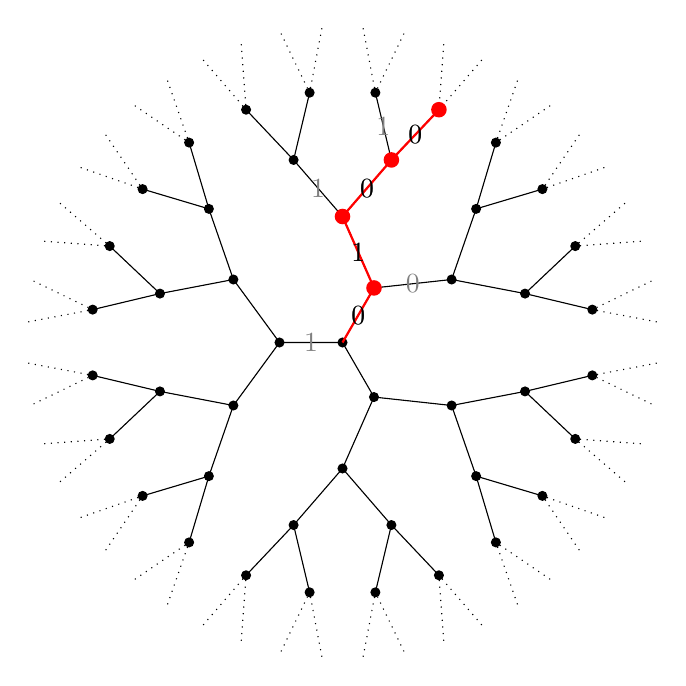
\begin{tikzpicture}[scale=0.8]
        \def\levels{5}
        \draw[fill] (0:0) circle (2pt);
        \foreach \i in {1,...,\levels} {
          \pgfmathparse{3*2^\i}
          \let\nodes\pgfmathresult
          \foreach \j in {1,3,...,\nodes} {
            \pgfmathparse{\j + (-1)^div(\j,2)}
            \let\lower\pgfmathresult
            \ifthenelse{\i = \levels}{
              \draw[dotted] (360/\nodes*\j : \i) --
              (360/\nodes*\lower : \i - 1);
            }{
              \draw[fill] (360/\nodes*\j : \i) circle (2pt) --
              (360/\nodes*\lower : \i - 1);
            }
          }
        }

        \def\h{4}
        \coordinate (DOWN) at (0:0);
        \foreach \x in {2,...,\levels} {
          \pgfmathparse{int(\x-1)}
          \let\i\pgfmathresult
          \pgfmathparse{3*2^\i}
          \let\nodes\pgfmathresult
          \pgfmathparse{div(\h, 2^(\levels-\x))}
          \let\u\pgfmathresult
          \pgfmathparse{int(mod(\u,2))}
          \let\bit\pgfmathresult
          \coordinate (UP) at ({360/\nodes*(2*\u+1)} : \i);
          \coordinate (N0) at ({360/\nodes*(2*(\u-\bit)+1)} : \i);
          \coordinate (N1) at ({360/\nodes*(2*(\u-\bit)+3)} : \i);
          \uncover<\i>{
            \draw[gray] ($(DOWN)!0.5!(N0)$) node {0} ($(DOWN)!0.5!(N1)$) node {1};
          }
          \uncover<\x->{
            \draw[fill,red,thick] (UP) circle (3pt) to node[black] {\bit} (DOWN);
          }
          \coordinate (DOWN) at (UP);
        }
      \end{tikzpicture}
    \end{column}
  \end{columns}
\end{frame}

%%


\begin{frame}[plain]
  \begin{beamercolorbox}[sep=0.1px,center,wd=\paperwidth,sep=0.5\paperheight]{palette tertiary}
    \Huge\centering Forensic categories

    \bigskip
    
    \normalsize(joint work with Basso, Patranabis, Radulescu, Wesolowski)
  \end{beamercolorbox}
\end{frame}

%%

\begin{frame}{Objects \uncover<2>{and Morphisms}}
  \centering
  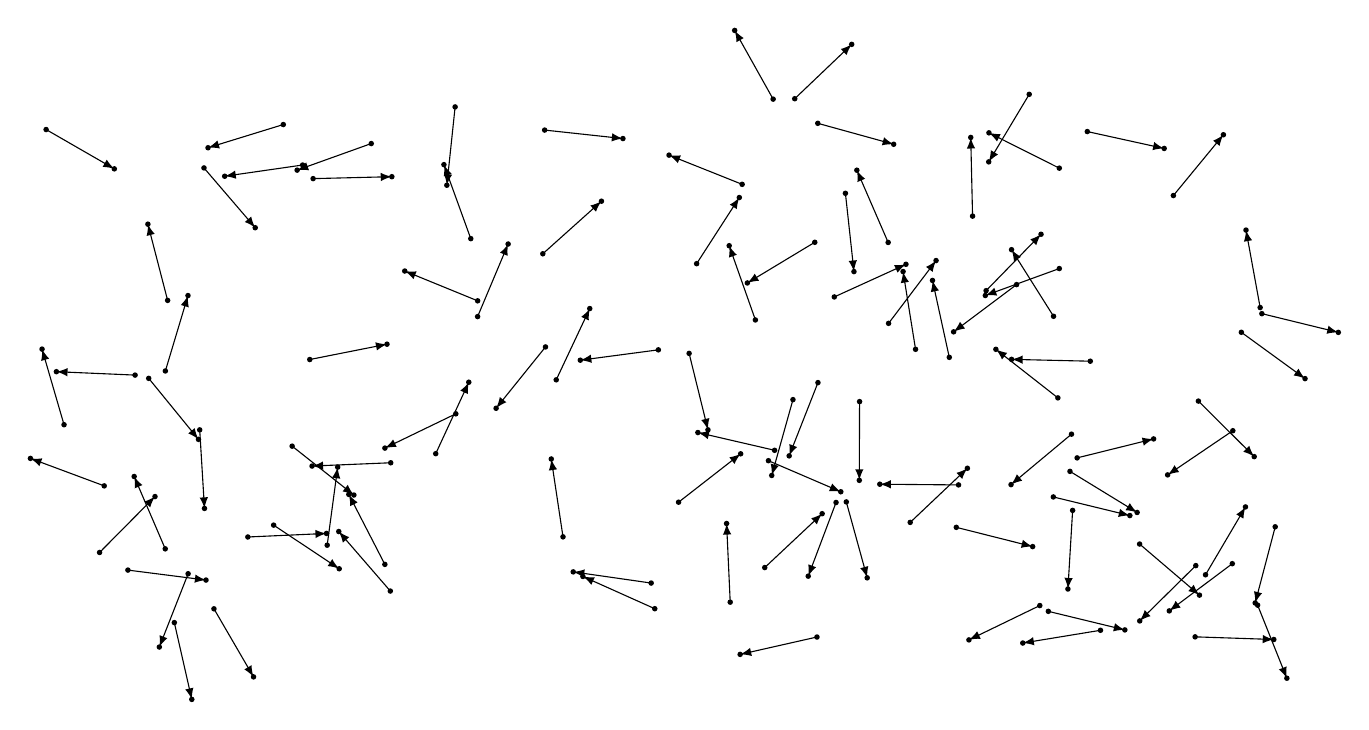
\begin{tikzpicture}
    \pgfmathsetseed{12345}
    \foreach \i in {1,...,100} {
      \pgfmathparse{16*random()}
      \let\x\pgfmathresult
      \pgfmathparse{7*random()}
      \let\y\pgfmathresult
      \pgfmathparse{360*random()}
      \let\ang\pgfmathresult
      \pgfmathparse{7*random()}
      \fill (\x,\y) circle (1pt) +(\ang:1) circle (1pt);
      \uncover<2>{\draw[-latex] (\x,\y) to +(\ang:1);}
    }
  \end{tikzpicture}  
\end{frame}

%%

\begin{frame}{More than graphs\dots}
  \begin{itemize}
  \item A finite set of \emph{objects} $\E$,
  \item For each pair $A,B\in\E$ a set of \emph{morphisms} $\Hom(A,B)$
  \end{itemize}

  \vfill
  
  \centering
  \begin{tikzpicture}
    \node (E1) at (0,0) {$B$};
    \node (E) at (6,0) {$A$};

    \draw[-latex] (E) edge node[above] {$φ$} (E1);
    \node at (3,-1.5) {$φ ∈ \Hom(A,B)$};

    \uncover<2->{
      \draw[-latex] (E) edge[loop,out=45,in=-45,looseness=10] node[right] {$ω$} (E);
      \node at (8,-1.5) {$ω ∈ \Hom(A,A)$};
    }
  \end{tikzpicture}
\end{frame}

%%

\begin{frame}{Transitively closed}
  \centering
  \begin{tikzpicture}
    \node (A) at (0,0) {$A$};
    \node (B) at (-6,0) {$B$};
    \node (C) at (-12,0) {$C$};

    \draw[-latex]
    (A) edge node[above] {$φ$} (B)
    (B) edge node[above] {$ψ$} (C);

    \uncover<2->{
      \draw[-latex]
      (A) edge[bend left] node[below] {$ψ∘φ$} (C);
    }
  \end{tikzpicture}
\end{frame}

%%

\begin{frame}{Identity morphisms}
  \centering
  \begin{tikzpicture}
    \node (A) at (0,0) {$A$};
    \node (B) at (-6,0) {$B$};
    \draw[-latex]
    (A) edge node[above] {$φ$} (B)
    (A) edge[loop,out=45,in=-45,looseness=10] node[right] {$1_A$} (A)
    (B) edge[loop,out=135,in=225,looseness=10] node[left] {$1_B$} (B);
    \node at (-3,-1.5) {$1_B∘φ \;=\; φ \;=\; φ∘1_A$};
  \end{tikzpicture}
\end{frame}

%% 


\begin{frame}{Computational axioms}
  \large
  \begin{itemize}
    \setlength{\itemsep}{2em}
  \item Every object and every morphism has a unique representation as
    a string;
  \item The representation of a morphism $\phi:A\to B$ identifies $A$
    and $B$;
  \item There exists efficient algorithms to verify that a string
    represents an object/morphism;
  \item There exists an \emph{origin object} $O \in \E$ whose
    representation is known;
  \item \dots
  \end{itemize}
\end{frame}

%%

\begin{frame}{Axiom: \textit{Walking}}
  \large
  Efficient algorithm for:
  
  \bigskip
  \begin{description}
  \item[Input:] Object $A$
  \item[Output:]
    \begin{itemize}
    \item Uniformly random object $B$,
    \item Random morphism $\phi:A\to B$.
    \end{itemize}
  \end{description}
\end{frame}

%%

\begin{frame}{Identification scheme?}
  \large
  \centering
  \begin{tikzpicture}
    \node (E0) at (0,0) {$O$};
    \node (Epk) at (8,0) {$A_{\mathrm{pk}}$};
    \uncover<2->{
      \node (Ecom) at (4,-5) {$B_{\mathrm{com}}$};
    }

    \draw[dashed,-latex]
    (E0) edge node[above]{secret key} (Epk);
    
    \uncover<2->{
      \draw[dashed,-latex]
      (E0) edge node[below,sloped]{random} (Ecom);
    }

    \uncover<3->{
      \draw[-latex] (Epk) edge node[below,sloped]{??} (Ecom);
    }
  \end{tikzpicture}
\end{frame}

%%

\begin{frame}{Axiom: Triangularizable}
  \centering
  \begin{tikzpicture}
    \node (O) at (0,0) {$O$};
    \node (A) at (2,-4) {$A$};
    \node (B) at (-2,-4) {$B$};
    \draw[-latex] (O) edge (A) edge (B);
    \node at (0,-5) {\emph{Input}};
    \uncover<2->{
      \node (AA) at (10,-4) {$A$};
      \node (BB) at (6,-4) {$B$};
      \draw[-latex] (AA) edge (BB);
      \node at (8,-5) {\emph{Output}};
    }
  \end{tikzpicture}
\end{frame}

%%

\begin{frame}{Identification scheme?}
  \large
  \centering
  \begin{tikzpicture}
    \node (E0) at (0,0) {$O$};
    \node (Epk) at (8,0) {$A_{\mathrm{pk}}$};
    \uncover<2->{
      \node (Ecom) at (4,-5) {$B_{\mathrm{com}}$};
    }

    \draw[dashed,-latex]
    (E0) edge node[above]{secret key} (Epk);
    
    \uncover<2->{
      \draw[dashed,-latex]
      (E0) edge node[below,sloped]{random} (Ecom);
    }

    \uncover<3->{
      \draw[-latex] (Epk) edge node[below,sloped]{random?} (Ecom);
    }
  \end{tikzpicture}
\end{frame}

%%

\begin{frame}{Hardness Assumption: \textit{Walk-indistinguishable}}
  \large
  These two distributions are indistinguishable:

  \vfill

  \begin{columns}
    \begin{column}{0.5\textwidth}
      \centering
      \begin{tikzpicture}
        \node (O) at (0,2) {};
        \node (A) at (1,0) {$A$};
        \node (B) at (-1,0) {$B$};
        \draw[-latex] (A) edge (B);
      \end{tikzpicture}

      \bigskip
      
      \begin{itemize}
      \item Given $A$,
      \item \emph{\textit{Walk} $\phi : A \to B$,}
      \end{itemize}
    \end{column}
    \begin{column}{0.5\textwidth}
      \centering
      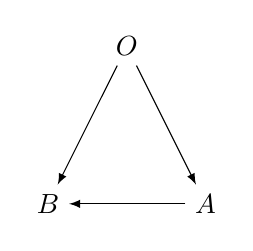
\begin{tikzpicture}
        \node (O) at (0,2) {$O$};
        \node (A) at (1,0) {$A$};
        \node (B) at (-1,0) {$B$};
        \draw[-latex] (O) edge (A) edge (B) (A) edge (B);
      \end{tikzpicture}

      \bigskip
      
      \begin{itemize}
      \item Given $O \to A$,
      \item Sample random $O \to B$,
      \item \emph{\textit{Triangularize} $\phi : A \to B$} 
      \end{itemize}
    \end{column}
  \end{columns}
\end{frame}

%%

\begin{frame}{Identification scheme?}
  \large
  \centering
  \begin{tikzpicture}
    \node (E0) at (0,0) {$O$};
    \node (Epk) at (8,0) {$A_{\mathrm{pk}}$};
    \uncover<2->{
      \node (Ecom) at (4,-5) {$B_{\mathrm{com}}$};
    }

    \uncover<2->{
      \draw[dashed,-latex]
      (E0) edge (Ecom);
    }

    \uncover<3->{
      \draw[-latex] (Epk) edge node[below,sloped]{??} (Ecom);
    }
  \end{tikzpicture}
\end{frame}

%%

\begin{frame}{Hardness assumption: \textit{Morphism Finding}}
  \large\centering
  Given two objects $A,B$, it is hard to find a morphism between them:

  \vfill
  
  \begin{tikzpicture}
    \node (A) at (4,0) {$A$};
    \node (B) at (-4,0) {$B$};
    \draw[dashed,-latex] (A) edge (B);
  \end{tikzpicture}

  \vfill
\end{frame}

%%

\begin{frame}{Summary}
  \large
  \begin{columns}
    \begin{column}{0.45\textwidth}
      \centering
      \begin{itemize}
        \setlength{\itemsep}{1em}
      \item \textit{Effective} category,
      \item Origin object $O$,
      \item Walking,
      \item Triangularizable,
      \item Walk-indistinguishable,
      \item Hard to find morphisms.
      \end{itemize}
    \end{column}
    \begin{column}{0.1\textwidth}
      \centering\Huge
      \[⇒\]
    \end{column}
    \begin{column}{0.45\textwidth}
      \centering
      GMW-style Identification scheme

      \bigskip
      
      \uncover<2->{
        \Large
        \alert{Lame!}
      }
    \end{column}
  \end{columns}
\end{frame}

%%

\begin{frame}{Towards a stronger hardness assumption}
  \centering\large
  \begin{tikzpicture}
    \node (A) at (4,0) {$A$};
    \node (B) at (-4,0) {$B$};
    \node at (0,0) {\alert{$≠$}};
    \draw[-latex]
    (A) edge[bend right] node[above] {$φ$} (B)
    edge [bend left] node[below] {$ψ$} (B);
  \end{tikzpicture}
\end{frame}

%%

\begin{frame}{Fingerprints}
  \Large
  \begin{itemize}
    \setlength{\itemsep}{2em}
  \item A finite set \emph{$\M$} with at least 2 elements
  \item Partial maps for any pair $A,B$:
    \[\fp \quad:\quad \Hom(A,B) \quad\to\quad \M \cup \{\bot\}\]
  \item<2-> Random walk $\to$ random fingerprint
  \end{itemize}
\end{frame}

%%

\begin{frame}{Hardness assumption: Forensic hardness}
  \centering\large It is hard to find a pair of morphisms $A\to B$
  with distinct fingerprints:

  \vfill
  
  \begin{tikzpicture}
    \node (A) at (4,0) {$A$};
    \node (B) at (-4,0) {$B$};
    \node at (0,0) {\alert{$\fp(φ) ≠ \fp(ψ)$}};
    \draw[-latex]
    (A) edge[bend right] node[above] {$φ$} (B)
    edge [bend left] node[below] {$ψ$} (B);
  \end{tikzpicture}

  \vfill
\end{frame}

%%

\begin{frame}{Easy corollary}
  \Large\centering
  Forensic hardness $\quad⇒\quad$ Hard to find morphisms
\end{frame}

%%

\begin{frame}{Axiom: Triangularizable (reloaded)}
  \centering
  \begin{tikzpicture}
    \node (O) at (0,0) {$O$};
    \node (A) at (2,-4) {$A$};
    \node (B) at (-2,-4) {$B$};
    \draw[-latex] (O) edge (A) edge (B);
    \node at (0,-5) {$m \in \M$};
    \node at (0,-6) {\emph{Input}};

    \node (AA) at (10,-4) {$A$};
    \node (BB) at (6,-4) {$B$};
    \draw[-latex] (AA) edge node[below] {$\fp(φ) = m$} (BB);
    \node at (8,-6) {\emph{Output}};
  \end{tikzpicture}
\end{frame}

%%

\begin{frame}{SQIsign (in Forensic categories)}
  \large
  \begin{columns}
    \begin{column}{0.6\textwidth}
      \centering
      \begin{tikzpicture}
        \node (E0) at (0,0) {$O$};
        \node (Epk) at (8,0) {$A_{\mathrm{pk}}$};
        \uncover<1-4>{
          \draw[dashed,-latex]
          (E0) edge node[above,sloped] {secret key} (Epk);
        }

        \uncover<2->{
          \node (Ecom) at (4,-5) {$B_{\mathrm{com}}$};
        }
        \uncover<2-4>{
          \draw[dashed,-latex]
          (E0) edge node[below,sloped] {random} (Ecom);
        }

        \uncover<3-4>{
          \foreach \i in {-40,-30,...,40} {
            \draw[dashed,-latex] (Epk) edge[bend right=\i] (Ecom);
          }
        }

        \uncover<4-> {
          \draw[-latex,thick] (Epk) edge[bend right=-10]
          node[above,sloped,fill=white] {$\fp(φ) = m$} (Ecom);
        }
      \end{tikzpicture}
    \end{column}
    \begin{column}{0.4\textwidth}
      \begin{description}
        \setlength{\itemsep}{1em}
      \item<2->[P:] generate random commitment \emph{$B_{\mathrm{com}}$}
      \item<4->[V:] challenge with random $m \in \M$
      \item<5->[P:] respond with
        \emph{$φ:A_{\mathrm{pk}} \to B_{\mathrm{com}}$}
        such that
        \emph{$\fp(φ) = m$}
      \end{description}
    \end{column}
  \end{columns}
\end{frame}

%%


\begin{frame}[plain]
  \begin{beamercolorbox}[sep=0.1px,center,wd=\paperwidth,sep=0.5\paperheight]{palette tertiary}
    \Huge\centering Isogenies, finally!
  \end{beamercolorbox}
\end{frame}

%%

\begin{frame}
  \Large
  \begin{description}
    \setlength{\itemsep}{4em}
  \item[Isogenies =] finite-kernel \textit{algebraic} group morphisms: \emph{$E \to E'$}
  \item[Endomorphisms =] isogenies \emph{$E \to E$}
  \end{description}
\end{frame}

%%

\begin{frame}
  \Large\centering
  \begin{tikzpicture}[remember picture,overlay,shift=(current page.center)]
    \node (E) at (-4,1) {\alt<1>{$E$}{$\bullet$}};
    \node (E1) at (4,1) {\alt<1>{$E'$}{$\bullet$}};
    \draw[-latex] (E) edge node[above] {\only<1>{$\phi$}} (E1);
    \uncover<3->{\node at (0,-1) {Isogenous};}
  \end{tikzpicture}
\end{frame}

%%

\begin{frame}
  \centering
  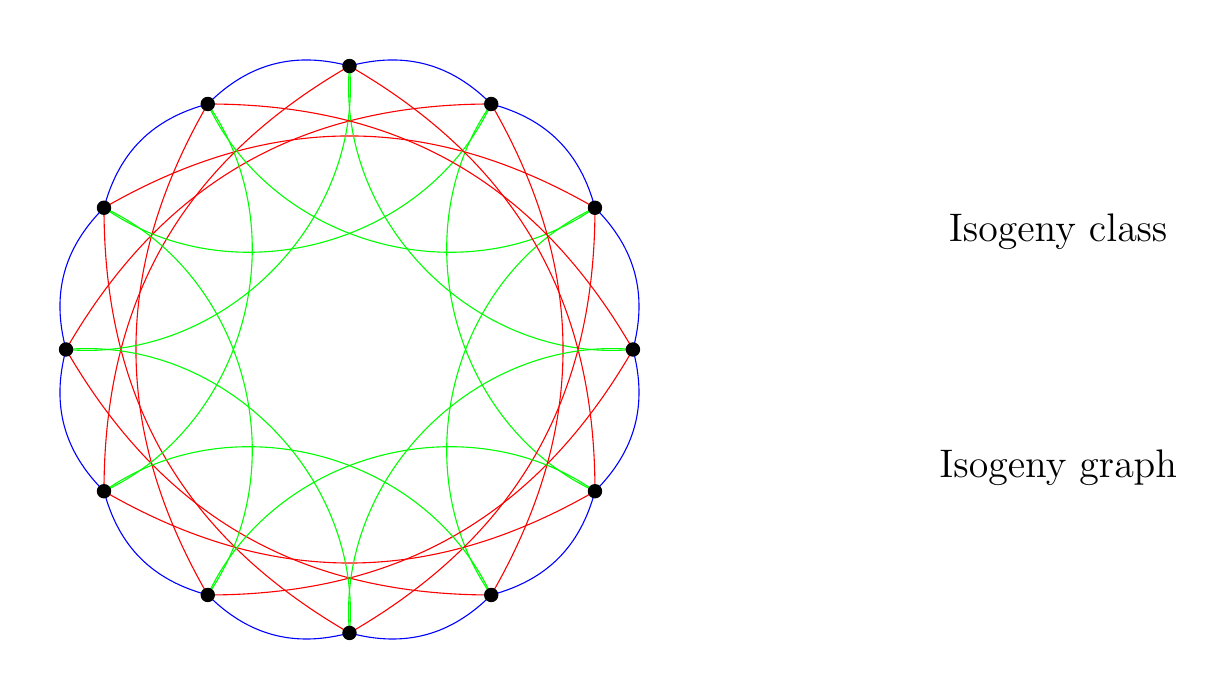
\begin{tikzpicture}
    \begin{scope}[scale=1.2]
      \def\crater{12}
      \def\jumpa{-8}
      \def\jumpb{9}
      \def\diam{3cm}

      \uncover<2->{
        \foreach \i in {1,...,\crater} {
          \draw[blue] (360/\crater*\i : \diam) to[bend right] (360/\crater*\i+360/\crater : \diam);
          \draw[red] (360/\crater*\i : \diam) to[bend right] (360/\crater*\i+\jumpa*360/\crater : \diam);
          \draw[green] (360/\crater*\i : \diam) to[bend right=50] (360/\crater*\i+\jumpb*360/\crater : \diam);
        }
      }
      \foreach \i in {1,...,\crater} {
        \draw[fill] (360/\crater*\i: \diam) circle (2pt) +(360/\crater*\i: 0.4);
      }
    \end{scope}

    \begin{scope}
      \Large
      \uncover<1->{\node at (9,1.5) {Isogeny class};}
      \uncover<2->{\node at (9,-1.5) {Isogeny graph};}
    \end{scope}
  \end{tikzpicture}
\end{frame}

%%

\begin{frame}{The isogeny problem}
  \Large\centering
  \begin{tikzpicture}
    \node (E) at (0,0) {$E$};
    \node (E1) at (8,0) {$E'$};
    \uncover<2->{
      \draw[-latex] (E) edge node[above] {??} (E1);
    }
  \end{tikzpicture}
\end{frame}

%% 

\begin{frame}{Anatomy of an isogeny}
  \transdissolve<2-8>
  \large
  \centering
  \begin{tikzpicture}
    \node at (-6,0) {$\phi(x,y) = \Biggl($};
    \node (x) at (-2.5,0) {$\displaystyle
      \frac{
        \only<-6>{x^4 - x^3 + 11x^2 + 9x + 12}
        \only<7->{g(x)}
      }{
        \only<-3>{\phantom{(}x^3-x^2-x+1\phantom{)}}
        \only<4-5>{(x + 1)(x - 1)^2}
        \only<6->{h(x)}
      },$};
    \node (y) at (3.5,0) {$\displaystyle y
      \only<-7>{\frac{x^5 - x^4 - 14x^3 - 26x^2 - 67x - 21}{x^5 - x^4 - 2x^3 + 2x^2 + x - 1}}
      \only<8->{\left(\frac{g(x)}{h(x)}\right)'}$};
    \node at (7,0) {$\Biggr)$};
    
    \begin{scope}[thick,red]
      \uncover<2-6>{\draw (-4.5,0.4) circle (0.2) +(0,0.2) -- +(0,1) +(0,1.2) node {degree};}
      \uncover<2>{\draw (-3.6,-0.2) circle (0.2) +(0,-0.2) -- +(0,-1) +(0,-1.2) node {degree $-1$};}
      \uncover<3-4>{
        \draw (-2.5,-0.3) ellipse (1.7 and 0.4) +(0,-0.4) -- +(0,-1.2) +(0,-1.4) node {kernel polynomial};
      }
      \uncover<5>{
        \draw (-3.3,-0.3) ellipse (0.7 and 0.4) +(-0.5,-0.3) -- +(-1,-0.6) +(-1.2,-0.8) node {Point of order $2$};
        \draw (-1.9,-0.3) ellipse (0.9 and 0.4) +(0.2,-0.4) -- +(1,-1.5) +(1.1,-1.7) node {Two points of order $4$};
      }
      \uncover<6->{
        \draw (-2.5,-0.6) -- +(0,-1) +(0,-1.5) node {$h(x) = \displaystyle\prod_{P\in K\setminus\{0\}}\bigl(x-x(P)\bigr)$};
      }
      \uncover<7->{
        \draw (-2.5,0.6) -- +(0,1) +(0,1.5) node {computed by Vélu--Elkies--Kohel formulas};
      }
    \end{scope}
  \end{tikzpicture}

  \medskip
  
  \begin{uncoverenv}<9->
    \begin{description}
    \item[Input:] Finite kernel \emph{$K⊂E$} of order \emph{$d$};
    \item[Output:] Rational fractions \emph{$ϕ(x,y)$};
    \item[Complexity:] \emph{$\tilde{O}(d)$} operations.
    \end{description}
  \end{uncoverenv}
\end{frame}

%%

\begin{frame}{Isogeny graphs}
  \large
  \begin{columns}
    \begin{column}{0.45\textwidth}
      \[
        \frac{x^2 + \cdots}{x + \cdots}
        \uncover<2->{\circ\frac{x^2 + \cdots}{x + \cdots}}
        \uncover<3->{\circ\frac{x^2 + \cdots}{x + \cdots}}
        \uncover<4->{\circ\frac{x^2 + \cdots}{x + \cdots}}
      \]
    \end{column}
    \begin{column}{0.55\textwidth}
      \centering
      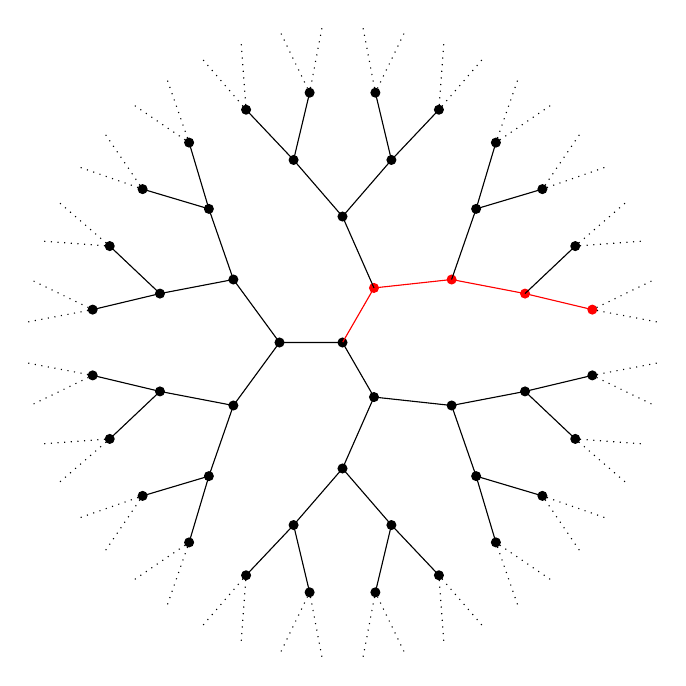
\begin{tikzpicture}[scale=0.8]
        \def\levels{5}
        \draw[fill] (0:0) circle (2pt);
        \foreach \i in {1,...,\levels} {
          \pgfmathparse{3*2^\i}
          \let\nodes\pgfmathresult
          \foreach \j in {1,3,...,\nodes} {
            \pgfmathparse{\j + (-1)^div(\j,2)}
            \let\lower\pgfmathresult
            \uncover<\i->{
              \ifthenelse{\i = \levels}{
                \draw[dotted] (360/\nodes*\j : \i) --
                (360/\nodes*\lower : \i - 1);
              }{
                \pgfextra{
                  \ifthenelse{\j=1}{\def\col{red}}{\def\col{black}}
                  \draw[fill,\col] (360/\nodes*\j : \i) circle (2pt) --
                  (360/\nodes*\lower : \i - 1);
                }
              }
            }
          }
        }
      \end{tikzpicture}
    \end{column}
  \end{columns}
\end{frame}

%%

\begin{frame}{Two computational worlds}
  \centering
  \setlength{\tabcolsep}{2em}
  \renewcommand{\arraystretch}{1.5}
  \begin{tabular}{p{0.3\textwidth} c c}
    & \textcolor{purple}{Quadratic imaginary} & \textcolor{red}{Quaternionic}\\
    \hline
    $\rank\Hom(E,E')$ & 2 & 4\\
    Endomorphism algebra & number field & quaternion algebra\\
    Maximal orders & one & many \\
    Ideal class\dots & \dots group & \dots set\\
    Find isogeny $E → E'$ & \alert{hard} & \alert{hard}\\
    Convert isogenies $\leftrightarrow$ ideals & easy\footnotemark[1] & easy\footnote[1]{When $\End(E)$ is known}\\
    Compute $\End(E)$ & easy & \alert{hard}\\
  \end{tabular}
\end{frame}

%%

\begin{frame}[plain]
  \begin{beamercolorbox}[sep=0.1px,center,wd=\paperwidth,sep=0.5\paperheight]{palette tertiary}
    \Huge\centering A cryptographic group action
  \end{beamercolorbox}
\end{frame}

%%

\begin{frame}{The quadratic imaginary case}
  \begin{block}{Complex Multiplication}
    Fix an order \emph{$\O ⊂ ℚ(\sqrt{-D})$}:
    \begin{itemize}
    \item Invertible ideal classes form a \emph{finite abelian group}
    \item $\Cl(\O)$ acts \emph{freely and transitively} on the set of
      elliptic curves with $\End(E) ≃ \O$.
    \end{itemize}
  \end{block}
\end{frame}

%%

\begin{frame}{Class group action}
  \begin{columns}
    \begin{column}{0.55\textwidth}
      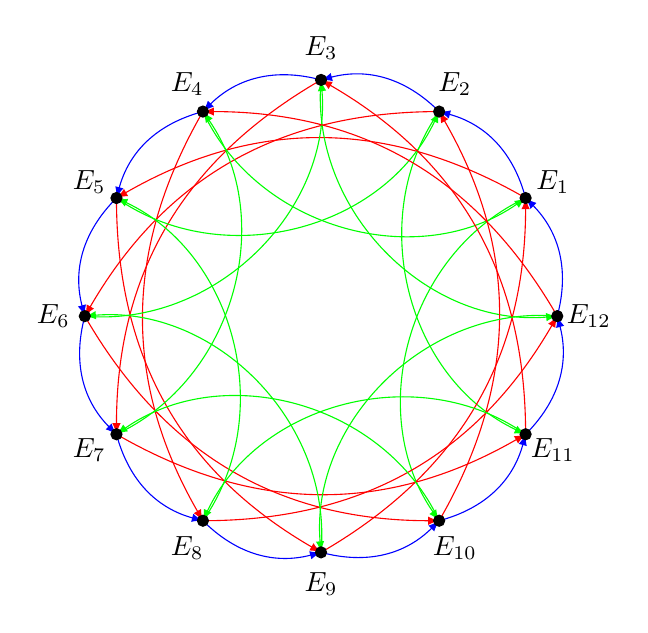
\begin{tikzpicture}
        \begin{scope}
          \def\crater{12}
          \def\jumpa{-8}
          \def\jumpb{9}
          \def\diam{3cm}

          \foreach \i in {1,...,\crater} {
            \draw[blue,-latex] (360/\crater*\i : \diam) to[bend right] (360/\crater*\i+360/\crater : \diam);
            \draw[red,-latex] (360/\crater*\i : \diam) to[bend right] (360/\crater*\i+\jumpa*360/\crater : \diam);
            \draw[green,-latex] (360/\crater*\i : \diam) to[bend right=50] (360/\crater*\i+\jumpb*360/\crater : \diam);
          }
          \foreach \i in {1,...,\crater} {
            \draw[fill] (360/\crater*\i: \diam) circle (2pt) +(360/\crater*\i: 0.4) node{$E_{\i}$};
          }
        \end{scope}
      \end{tikzpicture}
    \end{column}
    \begin{column}{0.45\textwidth}
      \large
      \begin{description}
        \setlength{\itemsep}{1em}
      \item<3->[Commutative]
        $E^{(\textcolor{red}{\bullet}\textcolor{blue}{\bullet})} = E^{(\textcolor{blue}{\bullet}\textcolor{red}{\bullet})}$
      \item<2->[Group]
        $((E^{\textcolor{blue}{\bullet}})^{\textcolor{red}{\bullet}})^{\textcolor{blue}{\bullet}} = E^{(\textcolor{blue}{\bullet}\textcolor{red}{\bullet}\textcolor{blue}{\bullet})} = E_1^{\textcolor{green}{\bullet}}$
      \item[Action]
        $E_2 = E_1^{\textcolor{blue}{\bullet}}$\\
        $E_5 = E_1^{\textcolor{red}{\bullet}}$\\
        $E_{10} = E_1^{\textcolor{green}{\bullet}}$
      \end{description}
    \end{column}
  \end{columns}
\end{frame}

%%

\begin{frame}{Two computational worlds}
  \centering
  \setlength{\tabcolsep}{2em}
  \renewcommand{\arraystretch}{1.5}
  \begin{tabular}{p{0.3\textwidth} c c}
    & \textcolor{purple}{Quadratic imaginary} & \textcolor{red}{Quaternionic}\\
    \hline
    $\rank\Hom(E,E')$ & 2 & 4\\
    Endomorphism algebra & number field & quaternion algebra\\
    Maximal orders & one & many \\
    Ideal class\dots & \dots group & \dots set\\
    Find isogeny $E → E'$ & \alert{hard} & \alert{hard}\\
    Convert isogenies $\leftrightarrow$ ideals & easy\footnotemark[1] & easy\footnote[1]{When $\End(E)$ is known}\\
    Compute $\End(E)$ & easy & \alert{hard}\\
  \end{tabular}
\end{frame}

%%

\begin{frame}[plain]
  \begin{beamercolorbox}[sep=0.1px,center,wd=\paperwidth,sep=0.5\paperheight]{palette tertiary}
    \Huge\centering A forensic category
  \end{beamercolorbox}
\end{frame}

%%

\begin{frame}{The Deuring correspondence (for supersingular curves)}
  \begin{block}{An equivalence of categories (roughly)}
    \centering
    \begin{tikzpicture}
      \node (O) at (0,0) {$\O$};
      \node (O1) at (6,0) {$\O'$};
      \node (E) at (0,-1) {$E$};
      \node (E1) at (6,-1) {$E'$};
      
      \begin{scope}[gray,anchor=north]
        \node (Oc) at (-2,1) {left order};
        \node at (-2, 1.5) {$\{ω\in B_{p,\infty}\;|\; ωI=I\}$};
        \node (O1c) at (8,1) {right order};
        \node at (8,1.5) {$\{ω\in B_{p,\infty}\;|\; Iω=I\}$};
        \node (ac) at (3,1.5) {connecting ideal};
        
        \node (Ec) at (-2,-2) {supersingular curve};
        \node (E1c) at (8,-2) {supersingular curve};
        \node (phic) at (3,-2) {isogeny};
      \end{scope}
      
      \draw[->] (O) edge node[auto] (a) {$I$} (O1)
      (E) edge node[auto,swap] (phi) {$\phi_I$} (E1);
      \draw[dashed,->] (Oc) edge (O) (O1c) edge (O1) (ac) edge (a)
      (Ec) edge (E) (E1c) edge (E1) (phic) edge (phi);
    \end{tikzpicture}
  \end{block}
\end{frame}

%%

\begin{frame}{The endomorphism ring problem}
  \Large\centering
  \vfill
  Given a random supersingular curve $E$, compute $\End(E)$
  \vfill
\end{frame}

%%

\begin{frame}{Contagious knowledge}
  \centering
  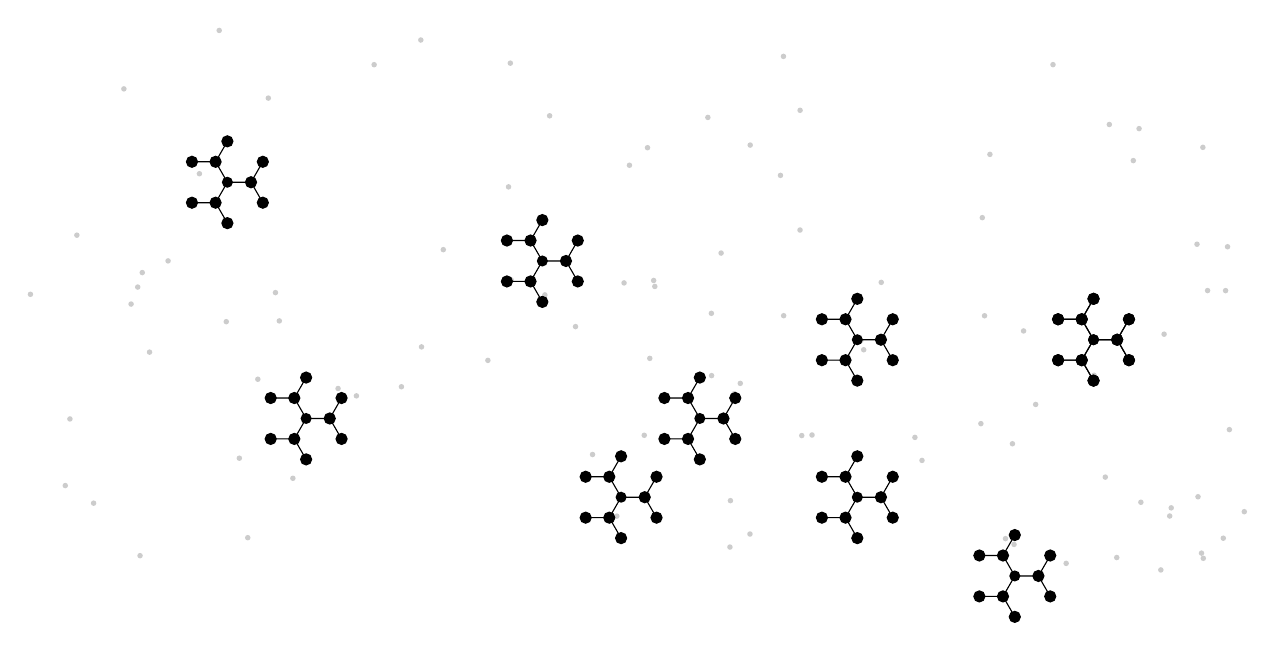
\begin{tikzpicture}
    \pgfmathsetseed{12345}
    \foreach \i in {1,...,100} {
      \pgfmathparse{16*random()}
      \let\x\pgfmathresult
      \pgfmathparse{7*random()}
      \let\y\pgfmathresult
      \fill[black!20!white] (\x,\y) circle (1pt);
    }
    \foreach \i in {1,...,10} {
      \pgfmathparse{floor(15*random())}
      \let\x\pgfmathresult
      \pgfmathparse{floor(6*random())}
      \let\y\pgfmathresult
      \fill (\x,\y) circle (2pt);
      \uncover<2->{
        \foreach \rho in {0,1,2} {
          \draw[fill,-latex] (\x,\y) -- +(120*\rho:.3) circle (2pt);
          \uncover<3->{
            \foreach \sigma in {-1,1} {
              \draw[fill,-latex] (\x,\y) ++(120*\rho:.3) -- ++(120*\rho+60*\sigma:.3) circle (2pt);
            }
          }
        }
      }
    }
  \end{tikzpicture}
\end{frame}

%%

\begin{frame}{$\End(E)$ as a trapdoor}
  \centering\large
  \setlength{\tabcolsep}{2em}
  \renewcommand{\arraystretch}{1.8}
  \begin{tabular}{c c c}
    Input & Output \\
    \hline
    random $E$ & $\End(E)$ & \alert{hard}\\
    random $E$ & $ω ∈ \End(E)$ & \alert{hard}\\
    random $E$ & $\phi : E_0\to E$ & \alert{hard}\\
    \hline
    $\End(E)$ & $E$ & easy\\
    $\End(E)$, $\End(E')$ & connecting ideal & easy\\
    \hline
    $I ⊂ \End(E)$ & $\phi_I : E → E'$ & easy\\
    $\End(E)$,\;\; $\phi: E → E'$ & $I_\phi ⊂ \End(E)$,\;\; $\End(E')$ & easy
  \end{tabular}
\end{frame}

%%

\begin{frame}{Axiom: \textit{Walking}}
  \begin{columns}
    \begin{column}{0.6\textwidth}
      \large
      Efficient algorithm for:
      
      \bigskip
      \begin{description}
      \item[Input:] Curve $A$
      \item[Output:]
        \begin{itemize}
        \item Uniformly random curve $B$,
        \item Random isogeny $\phi:A\to B$.
        \end{itemize}
      \end{description}
    \end{column}
    %%
    \begin{column}{0.4\textwidth}
      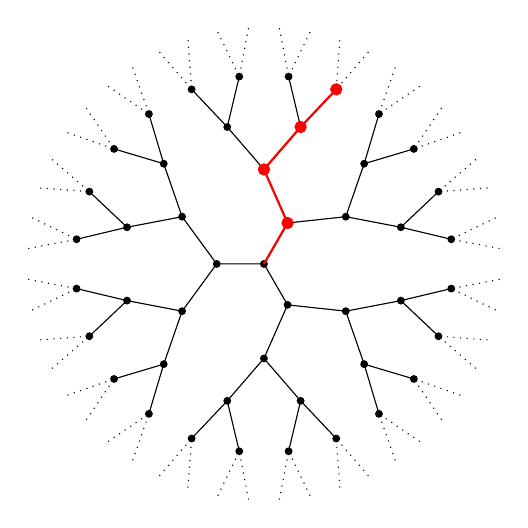
\begin{tikzpicture}[scale=0.6]
        \def\levels{5}
        \draw[fill] (0:0) circle (2pt);
        \foreach \i in {1,...,\levels} {
          \pgfmathparse{3*2^\i}
          \let\nodes\pgfmathresult
          \foreach \j in {1,3,...,\nodes} {
            \pgfmathparse{\j + (-1)^div(\j,2)}
            \let\lower\pgfmathresult
            \ifthenelse{\i = \levels}{
              \draw[dotted] (360/\nodes*\j : \i) --
              (360/\nodes*\lower : \i - 1);
            }{
              \draw[fill] (360/\nodes*\j : \i) circle (2pt) --
              (360/\nodes*\lower : \i - 1);
            }
          }
        }

        \def\h{4}
        \coordinate (DOWN) at (0:0);
        \foreach \x in {2,...,\levels} {
          \pgfmathparse{int(\x-1)}
          \let\i\pgfmathresult
          \pgfmathparse{3*2^\i}
          \let\nodes\pgfmathresult
          \pgfmathparse{div(\h, 2^(\levels-\x))}
          \let\u\pgfmathresult
          \pgfmathparse{int(mod(\u,2))}
          \let\bit\pgfmathresult
          \coordinate (UP) at ({360/\nodes*(2*\u+1)} : \i);
          \coordinate (N0) at ({360/\nodes*(2*(\u-\bit)+1)} : \i);
          \coordinate (N1) at ({360/\nodes*(2*(\u-\bit)+3)} : \i);
          \draw[fill,red,thick] (UP) circle (3pt) to (DOWN);
          \coordinate (DOWN) at (UP);
        }
      \end{tikzpicture}
    \end{column}
  \end{columns}
\end{frame}

%%

\begin{frame}{Axiom: Triangularizable}
  \centering
  \begin{tikzpicture}
    \node (O) at (0,0) {$O,\End(O)$};
    \node (A) at (2,-4) {$A\uncover<2->{,\End(A)}$};
    \node (B) at (-2,-4) {$B\uncover<2->{,\End(B)}$};
    \draw[-latex] (O) edge (A) edge (B);
    \node at (0,-5) {\emph{Input}};
    \uncover<3->{
      \node (AA) at (10,-4) {$A$};
      \node (BB) at (6,-4) {$B$};
      \draw[-latex] (AA) edge node[above] {{\uncover<4->{\small walk-indistinguishable}}} (BB);
      \node at (8,-5) {\emph{Output}};
    }
  \end{tikzpicture}
\end{frame}

%%

\begin{frame}{Fingerprints}
  \large
  \begin{center}
    \begin{tikzpicture}
      \node (A) at (0,0) {$E$};
      \node (B) at (-6,0) {$E'$};
      \draw[-latex] (A) edge node[above]{$φ$} (B);
    \end{tikzpicture}
  \end{center}

  \bigskip
  
  How the isogeny acts on points of order $N$:

  \bigskip
  
  \begin{description}
    \setlength{\itemsep}{1em}
  \item[Kernel fingerprint:] $\ker φ \cap E[N]$\\
    \hfill{\small(OG SQIsign)}
  \item[Level fingerprint:] Action on fixed bases of $E[N]$ and $E'[N]$\\
    \hfill{\small(joint with Borin, Lido, Schaeffler)}
  \end{description}
\end{frame}

%%

\begin{frame}{Worth the effort?}

  \centering

  \textbf{SQIsign v2 (June 2025)}
  \begin{table}[h]
    \centering
    \begin{tabular}{c r r r r r}
      \toprule
      & \multicolumn{2}{c}{Sizes (bytes)} & \multicolumn{3}{c}{Timings (ms)}\\
      \cmidrule(lr){2-3}\cmidrule(lr){4-6}
      Security & Public Key & Signature & Keygen & Sign & Verify \\
      \midrule
        NIST-1 &  66 & 148 &  25 &   60 &  3 \\
        NIST-3 &  98 & 222 &  67 &  161 &  9 \\
        NIST-5 & 130 & 294 & 119 &  300 & 18 \\
      \bottomrule
    \end{tabular}
  \end{table}  
\end{frame}

%%

\begin{frame}{What crypto from isogenies?}
  \small
  \renewcommand{\arraystretch}{1.5}
  \begin{tabular}{p{0.15\textwidth} p{0.25\textwidth} p{0.25\textwidth} p{0.25\textwidth}}
    & \emph{Key exchange / Encryption} & \emph{Identification / Signature} & \emph{Other}\\
    \hline
    \emph{Quadratic}\par \emph{(Group actions)}
    & Couveignes--Rostovtsev--Stolbunov\par CSIDH\par SCALLOP
                                & SeaSign\par CSI-FiSh\par PEGASIS
                                                             & Threshold\par PAKE\par \dots\\
    \emph{Quaternionic}\par \emph{\footnotesize(Forensic cat.)}
    & ---
                                & \strut\emph{SQIsign}\par SIDH-like signatures
                                                             & Ring signatures\par Adaptor signatures\par Chameleon hash\par \dots\\
    \emph{\textit{Ad hoc}\par \emph{\footnotesize(Level structures)}}
    & \strut\alert{SIDH~$\dagger$}\par SIDH fixes\par FESTA
                                & SIDH-like signatures
                                                             & Time-release crypto\par\dots
  \end{tabular}
\end{frame}

%%

\begin{frame}[plain]
  \centering
  \begin{tikzpicture}[remember picture,overlay]
    \begin{scope}[xscale=1.7,yshift=-15,opacity=0.8]
      \def\crater{12}
      \def\jumpa{-8}
      \def\jumpb{9}
      \def\diam{5cm}

      \foreach \i in {1,...,\crater} {
        \draw[blue] (360/\crater*\i : \diam) to[bend right] (360/\crater*\i+360/\crater : \diam);
        \draw[red] (360/\crater*\i : \diam) to[bend right] (360/\crater*\i+\jumpa*360/\crater : \diam);
        \draw[green] (360/\crater*\i : \diam) to[bend right=50] (360/\crater*\i+\jumpb*360/\crater : \diam);
      }
    \end{scope}
    
    \draw (0,0.5) node{\Huge\bf Thank you};
    \draw (0,-0.6) node{\large\url{https://defeo.lu/}};
    \draw (0,-1.3) node{\large\includegraphics[height=0.9em]{mastodon.png}~\href{https://twitter.com/luca_defeo}{@luca\_defeo@ioc.exchange}};
    \draw (0,-1.9) node{\large\includegraphics[height=0.9em]{bluesky.png}~\href{https://bsky.app/profile/bsky.defeo.lu}{@bsky.defeo.lu}};
  \end{tikzpicture}
\end{frame}

\end{document}


% LocalWords:  Isogeny abelian isogenies hyperelliptic supersingular Frobenius
% LocalWords:  isogenous
